% Created 2017-04-22 Sat 19:37
\documentclass[presentation]{beamer}
\usepackage[utf8]{inputenc}
\usepackage[T1]{fontenc}
\usepackage{fixltx2e}
\usepackage{graphicx}
\usepackage{longtable}
\usepackage{float}
\usepackage{wrapfig}
\usepackage{rotating}
\usepackage[normalem]{ulem}
\usepackage{amsmath}
\usepackage{textcomp}
\usepackage{marvosym}
\usepackage{wasysym}
\usepackage{amssymb}
\usepackage{hyperref}
\tolerance=1000
\usetheme{Madrid}
\author{Maxim Litvak}
\date{22 April, 2017}
\title{Finance through algorithmic lens}
\hypersetup{
  pdfkeywords={},
  pdfsubject={},
  pdfcreator={Emacs 25.1.1 (Org mode 8.2.10)}}
\begin{document}

\maketitle
\begin{frame}{Outline}
\tableofcontents
\end{frame}

\section{Outline}
\label{sec-1}
\begin{frame}[label=sec-1-1]{Outline}
\begin{block}{1st half - build algorithmic lens}
\begin{itemize}
\item We'll get the fast overview of fundmentals of algortihms
\item Take-aways: 1 picture, 2 paradoxes, a few example algorithms
\end{itemize}
\end{block}
\begin{block}{2nd half - look through it on finance}
\begin{itemize}
\item 3 practical cases
\item Some theoretical insights
\item Blockchain
\item Auctions
\item Non-monetary algorithms
\end{itemize}
\end{block}
\end{frame}
\section{Algorithms}
\label{sec-2}
\begin{frame}[label=sec-2-1]{Example: find an atom in the universe}
\begin{itemize}
\item How fast can we find a specific atom in the universe?
\item The current estimate is that there are $10^{80}$ ($\approx2^{270}$) atoms in the universe.
\item Sounds like a needle in a haystack at least \ldots{}
\end{itemize}
\end{frame}
\begin{frame}[label=sec-2-2]{Example: find an atom in the universe}
\begin{block}{1st attempt}
\begin{itemize}
\item Check each atom if it's the right one
\item With some luck, the 1st guess works
\item With no luck, the last guess works (after $10^{80}$ guess operations)
\item On average we'd need $5*10^79$ operations
\item Can we do better than this?
\end{itemize}
\end{block}
\end{frame}
\begin{frame}[label=sec-2-3]{Example: find an atom in the universe}
\begin{block}{Algorithm}
\begin{itemize}
\item Split the universe in 2 halves: in which half is the atom we need?
\item Repeat
\end{itemize}
\end{block}
\begin{block}{Result}
\begin{itemize}
\item In 270 operations we'll find it
\item Could be done by hand in less than 5 minutes \ldots{}
\item We've seen an algorithm being extremely fast on a large input
\end{itemize}
\end{block}
\end{frame}
\begin{frame}[label=sec-2-4]{Example: Hanoi tower}
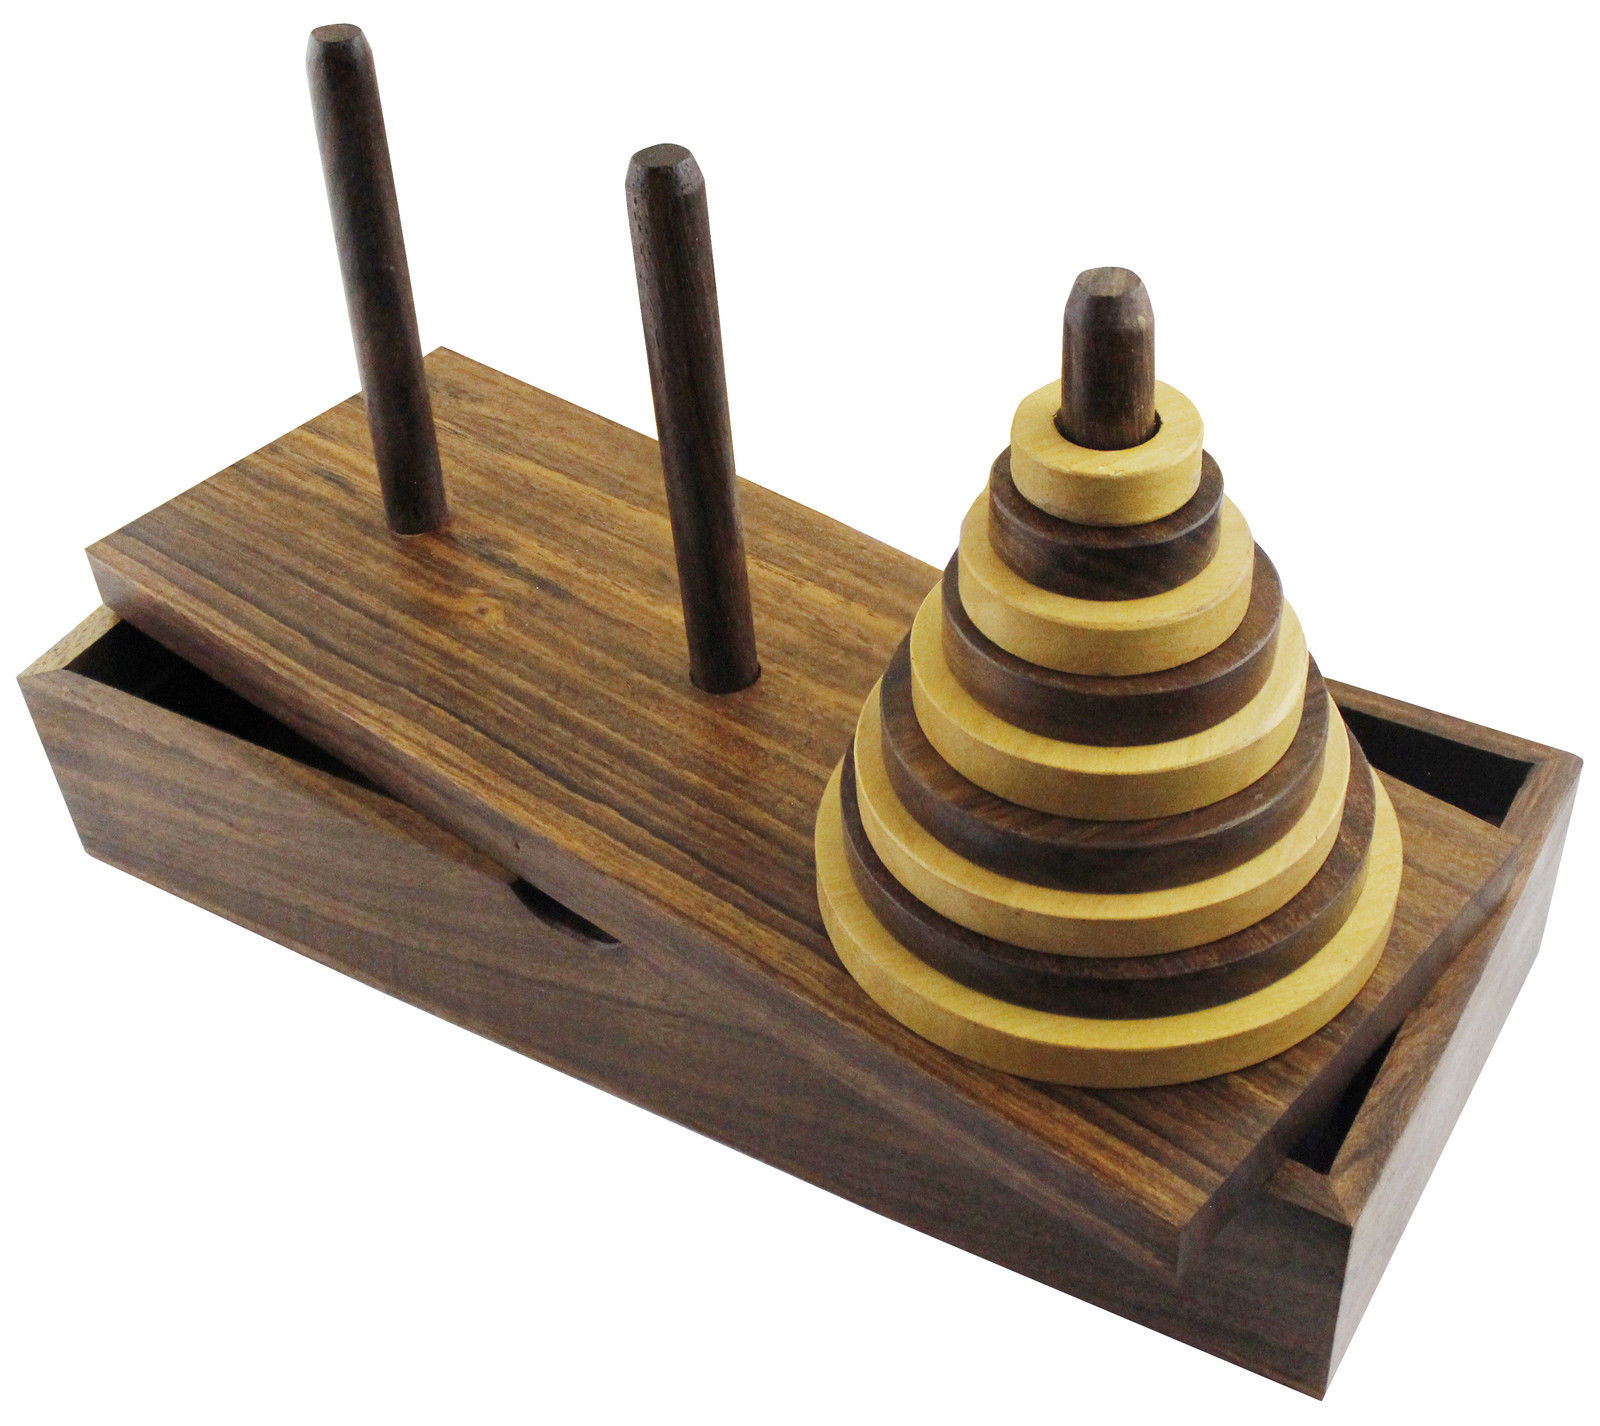
\includegraphics[width=.9\linewidth]{./img/tower_hanoi2.jpg}
\end{frame}
\begin{frame}[label=sec-2-5]{Example: Hanoi tower}
\begin{block}{Task}
Move all disks from one peg (tower) to another
\end{block}
\begin{block}{Rules:}
\begin{itemize}
\item 1. Move one disk at a time
\item 2. Every disk must be bigger than the one below
\item 3. You can move only the upper disk
\end{itemize}
\end{block}
\end{frame}
\begin{frame}[label=sec-2-6]{Example: Hanoi tower}
\begin{itemize}
\item 3 moves needed for 2 disks
\item 7 moves are needed for 3 disks
\item 15 moves are needed for 4 disks
\item \ldots{} million moves for 20 disks
\item Number of moves goes up exponentially with number of disks!
\end{itemize}
\end{frame}
\begin{frame}[label=sec-2-7]{Example: Hanoi tower}
\begin{itemize}
\item We've seen a task with an algorithm that is fast on huge input (atom searching)
\item We've seen a task with an algorithm that is slow on small input (Hanoi tower)
\end{itemize}
\end{frame}
\begin{frame}[label=sec-2-8]{Picture to take away}
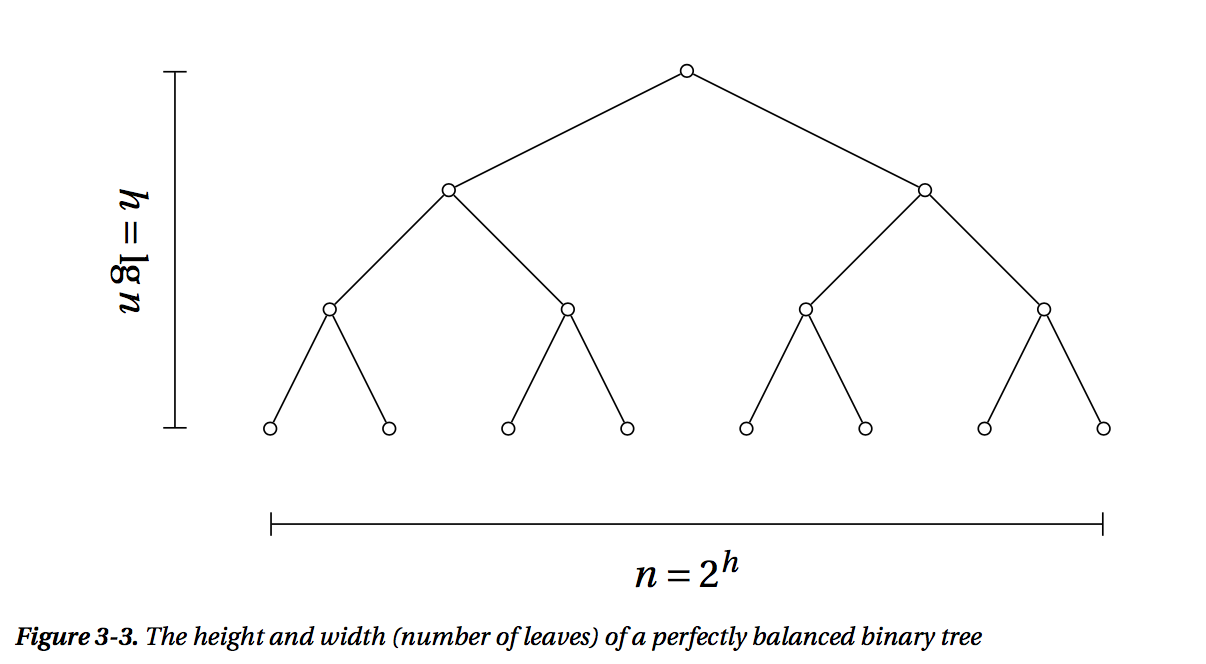
\includegraphics[width=.9\linewidth]{./img/bintree.png}
\begin{itemize}
\item The height is \alert{log(n)} (fast), the width is \alert{$n=2^h$}, the number of nodes is \alert{$2n - 1 = 2^{h+1} - 1$} (slow)
\end{itemize}
\end{frame}
\begin{frame}[label=sec-2-9]{Picture to take away}
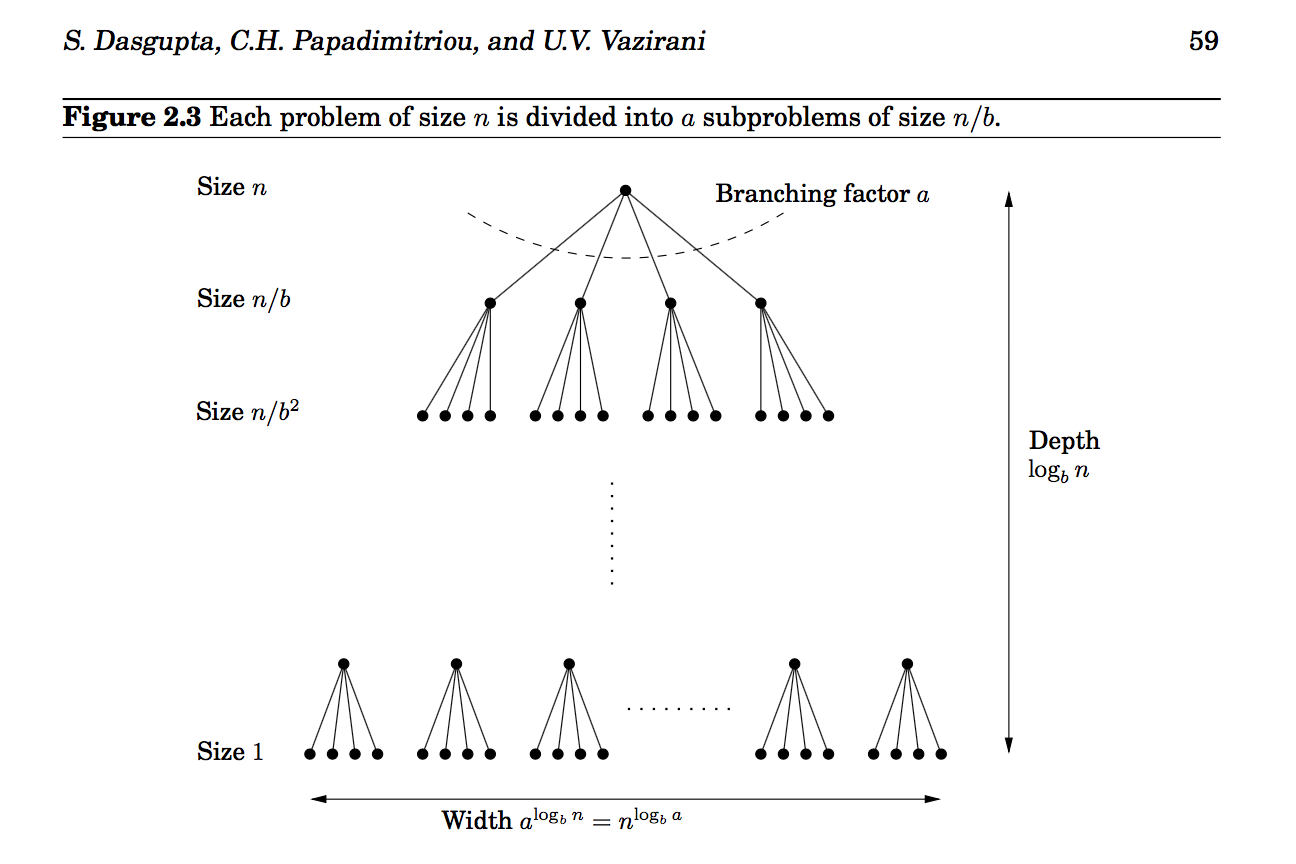
\includegraphics[width=.9\linewidth]{./img/tree2.png}
\end{frame}
\begin{frame}[label=sec-2-10]{Paradoxes - Multiplication}
\begin{block}{It's possible to multiply 2 numbers faster than the school method}
\begin{itemize}
\item Andrey Kolmogorov in 1960 conjectured that there's no multiplication method faster than the school method (used by the humanity for thousands of years), and organized seminar to prove it
\item A 17 years old student (Anatoly Karatsuba) found a faster method \ldots{}
\end{itemize}
\end{block}
\end{frame}
\begin{frame}[label=sec-2-11]{Paradoxes - Multiplication}

\includegraphics[width=.9\linewidth]{./img/gwh-problem-posing.jpg}
\end{frame}
\begin{frame}[label=sec-2-12]{Paradoxes - Multiplication}
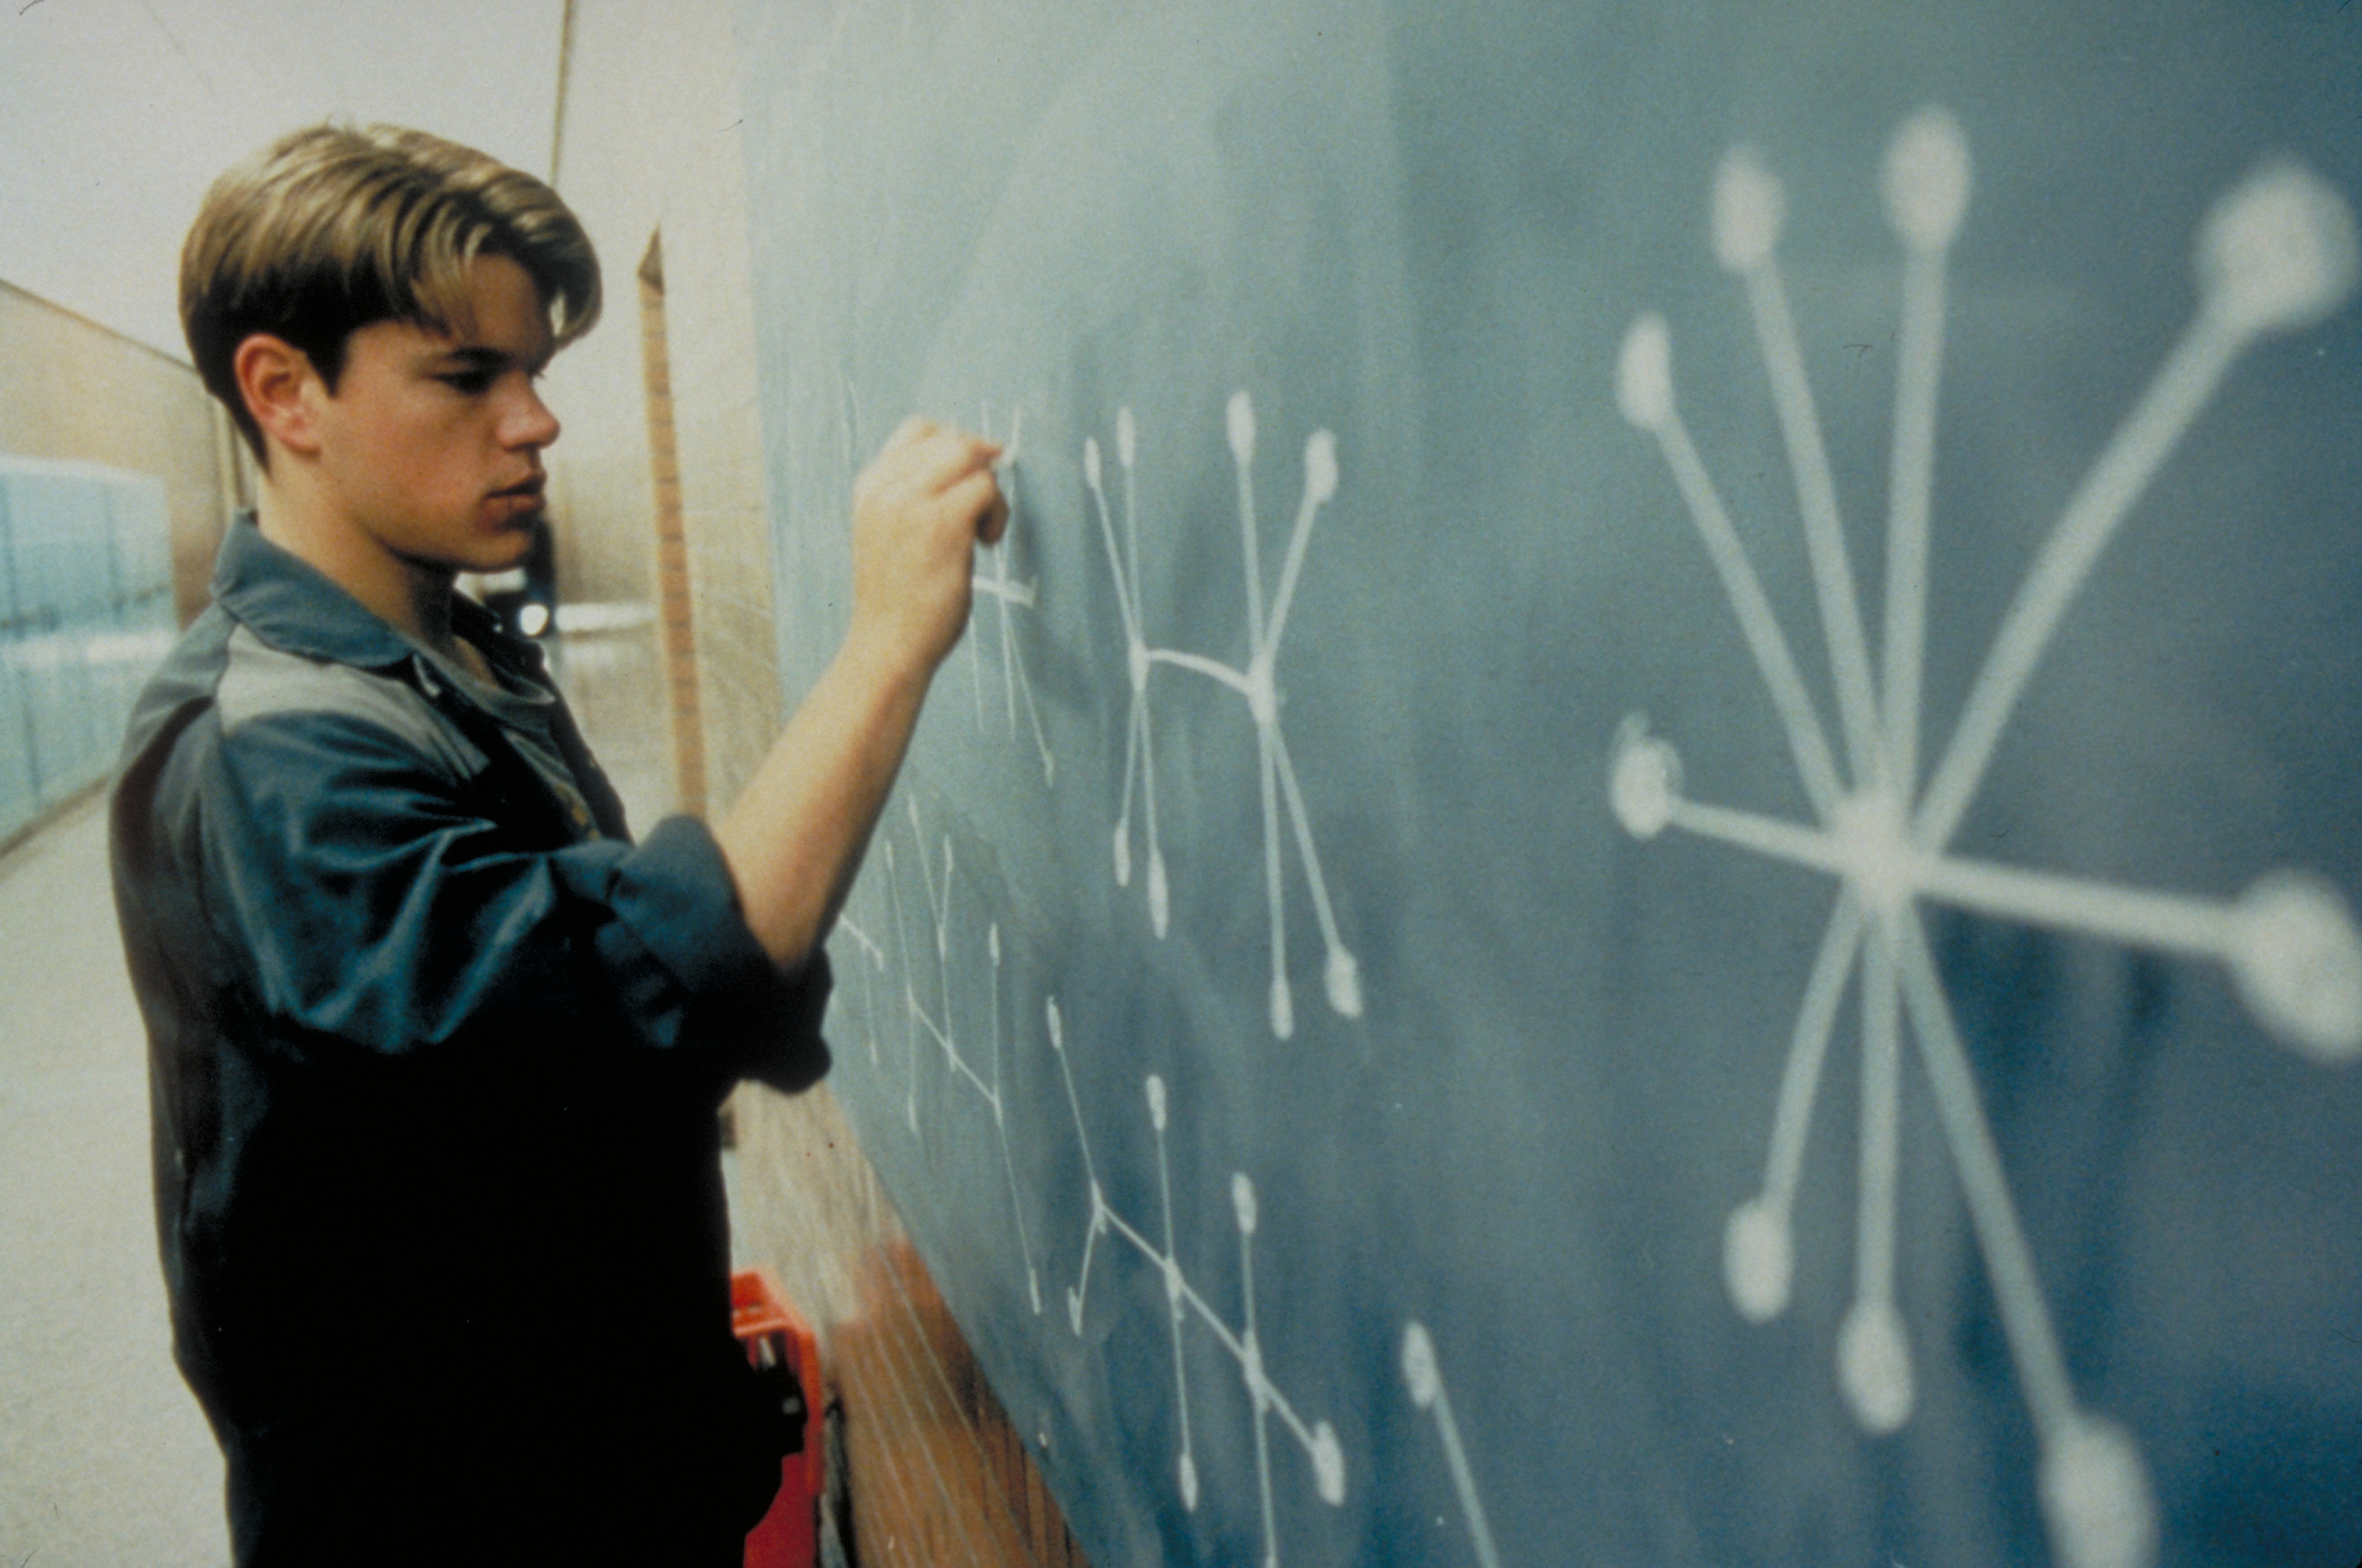
\includegraphics[width=.9\linewidth]{./img/gwh-problem-solving.jpg}
\end{frame}
\begin{frame}[label=sec-2-13]{Paradoxes - Multiplication}
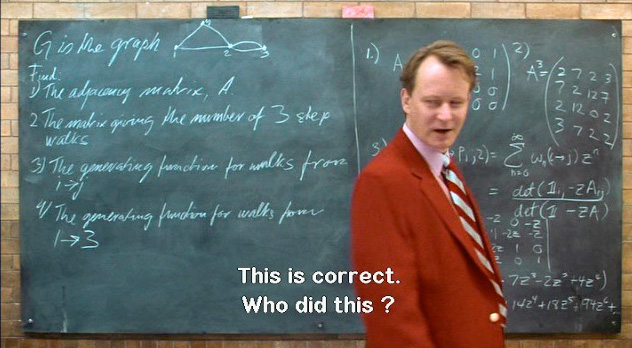
\includegraphics[width=.9\linewidth]{./img/gwh-solution-validated.jpg}
\end{frame}
\begin{frame}[label=sec-2-14]{Paradoxes - Multiplication}

\includegraphics[width=.9\linewidth]{./img/gwh-not-your-fault.jpg}
\end{frame}
\begin{frame}[fragile,label=sec-2-15]{Paradoxes - Multiplication}
 \begin{block}{School}
\begin{verbatim}
 25 
x
 17 
 ---
 175 
+
 25 
 ---
 425
\end{verbatim}
$(2\times10 + 5)(1\times10 + 7) = (2\times1)\times100 + (2\times7 + 5\times1)\times10 + (5\times7)\times1 = 425$
\end{block}
\end{frame}
\begin{frame}[fragile,label=sec-2-16]{Paradoxes - Multiplication}
 \begin{block}{Karatsuba}
\begin{verbatim}
(2*10 + 5)(1*10 + 7) = x*100 + y*10 + z*1 = ...
----------------------
x = 2*1 = 2
z = 5*7 = 35
y = (2 + 5)*(1 + 7) - (x + z) = 56 - 37 = 19
----------------------
... = 2*100 + 19*10 + 35*1 = 425
\end{verbatim}
\end{block}
\end{frame}
\begin{frame}[label=sec-2-17]{Paradoxes - Multiplication}
\begin{block}{Difference}
\begin{itemize}
\item School method - 4 multiplications and some additions
\item Karatsuba method - 3 multiplications and some more additions
\item Karatsuba is faster because the recursion can be deployed on multiplication
\end{itemize}
\end{block}
\end{frame}
\begin{frame}[label=sec-2-18]{Paradoxes - Braess paradox}
\begin{itemize}
\item Decreasing the number of opportunities might increase the efficiency
\item In option pricing - adding an opportunity can't reduce the price
\end{itemize}
\end{frame}
\begin{frame}[label=sec-2-19]{Paradoxes - Braess paradox}
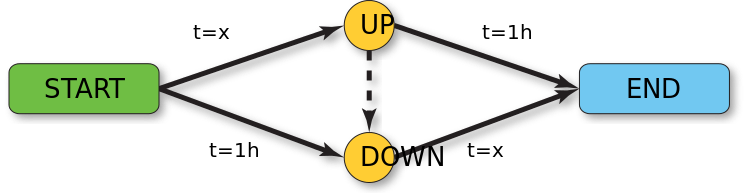
\includegraphics[width=.9\linewidth]{./img/braess.png}
\begin{itemize}
\item The roads START-DOWN and UP-END take 1 hour, the roads S-up and Down-t depend on traffic (100\% cars on the road - 1 hour, 50\% - 30min)
\item Initial equilibrium - 1.5h trip time (one half goes the upper way)
\item Adding high-speed UP-DOWN highway (with 0h time to cross it) increases the time to 2h
\end{itemize}
\end{frame}
\begin{frame}[label=sec-2-20]{What is "fast"}
\begin{itemize}
\item From algorithmic point of view, under the "speed" is considered the asymptotic behaviour of the algorithm on input
\item For a certain input, algorithm A might be faster than B, but "slower" in the asymptotic sense, i.e. with input big enough B outperforms A
\item Big-O notation: f(n) = O(g(n)) if (up to a constant) for some n,  g(n) catches up or outperforms f(n)
\end{itemize}
\end{frame}
\begin{frame}[label=sec-2-21]{What is "fast"}
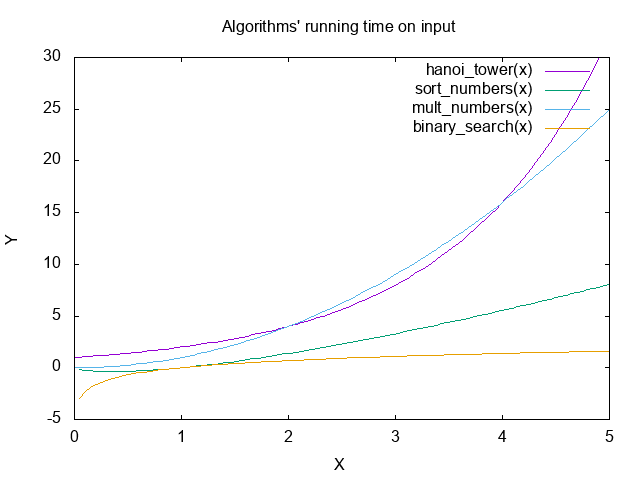
\includegraphics[width=.9\linewidth]{file.png}
\end{frame}

\begin{frame}[label=sec-2-22]{What is "hard" to compute}
\begin{itemize}
\item As a rule of thumb, the algorithms that can be computed in polynomial time are considered as "\alert{easy}" to compute
\item \ldots{} and algorithms which computation time can't be bound by a polynom (e.g. exponential) are considered to be "\alert{hard}"
\item Sometimes computational "hardness" is a good thing, if you don't want something to be easily computed (e.g. cryptography)
\item A lot of "hard" algorithms are considered to be "hard" since no faster solution is known (includes P = NP problem)
\end{itemize}
\end{frame}
\begin{frame}[label=sec-2-23]{Examples of algorithm's speed (current stand)}
\begin{itemize}
\item Sorting numbers - O(n log(n))
\item Binary search - O(log(n))
\item Satifiability (if some logical statement is true or not) - exponential
\item Integer number factorization (important in cryptography) - exponential
\end{itemize}
\end{frame}
\begin{frame}[label=sec-2-24]{Non-standard examples on complexity \ldots{}}
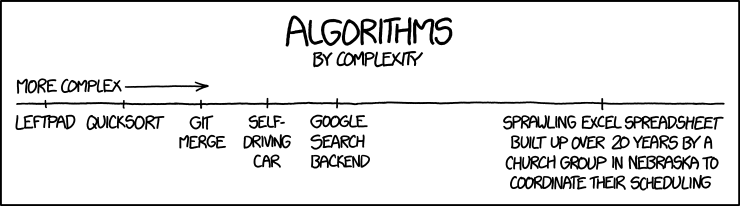
\includegraphics[width=.9\linewidth]{./img/xkcd_alg.png}
\begin{itemize}
\item xkcd.com
\end{itemize}
\end{frame}
\section{Finance}
\label{sec-3}
\begin{frame}[label=sec-3-1]{Algorithmic topics in finance}
\begin{itemize}
\item Cases in practice of quantitative finance
\item Theoretical insights
\item Blockchain
\item Auctions
\item Non-monetary mechanisms
\end{itemize}
\end{frame}
\begin{frame}[label=sec-3-2]{Case: generate normal r.v.}
\begin{itemize}
\item We can generate a normally distributed r.v. in a few ways, not all of them are equal computationally
\end{itemize}
\begin{block}{(Bad solution)}
\begin{itemize}
\item Generate 1000 uniformly distributed r.v. and use the CLT
\item Their sum (centered by mean and normalized by standard deviation) is (approximately) normally distributed
\item However, it's computationally expensive to do it this way
\end{itemize}
\end{block}
\end{frame}
\begin{frame}[label=sec-3-3]{Case: generate normal r.v.}
\begin{block}{Another solution:}
\begin{itemize}
\item use inverse c.d.f.
\item $\xi = \Phi^{-1}(\eta)$, s.t. $\eta \in U_{0,1}$
\item Next question: how expensive is it to compute inverse c.d.f.?
\end{itemize}
\end{block}
\begin{block}{Subproblem: computation of inverse c.d.f.}
\begin{itemize}
\item Option: calculate using the root-finding procedure (on average 5-6 iterations, however, in this case the c.d.f. itself might be costly to compute)
\item Option: use the Taylor expansion (well explored for normal distribution, might not be the case for other distributions)
\end{itemize}
\end{block}
\end{frame}
\begin{frame}[label=sec-3-4]{Case: generate normal r.v.}
\begin{itemize}
\item Other methods are known (Box-Miller procedure etc)
\item However, the very 1st question: how costly is it to compute pseudo-random uniformly distributed r.v.?
\item (guess) r.v. generators with better properties might be harder to compute
\end{itemize}
\end{frame}
\begin{frame}[label=sec-3-5]{Case: generate normal r.v.}
\begin{itemize}
\item Fast, but not so efficient generator \ldots{} (xkcd.com)
\end{itemize}
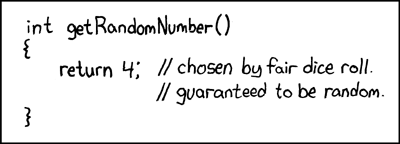
\includegraphics[width=.9\linewidth]{./img/xkcd_random.png}
\end{frame}
\begin{frame}[label=sec-3-6]{Case: generate normal r.v.}
\begin{itemize}
\item Example: middle square method
\item Simple, but has different flaws
\item Was enough for the simulations for the 1st nuclear bomb
\end{itemize}
\begin{block}{middle square method}
\begin{itemize}
\item Start with some n-digit number
\item Square it
\item Take the middle as the next number in the sequence
\item Example: $6234^2$ -> $38\underline{8627}56$, i.e. next number is 8627
\item Problem: $7600^2$ -> $57\underline{7600}00$, i.e. generator got stuck at the same number
\item For 4 digits maximal period is $2^{12}$ (one of modern generators has the period $2^{19937}$)
\end{itemize}
\end{block}
\end{frame}
\begin{frame}[label=sec-3-7]{Case: credit pricing}
\begin{itemize}
\item A big bank re-calculated for controlling purposes each month its whole portfolio of credits ($10^6$ credits)
\item For a lot of credits you need to do the same calculation (e.g. credits with the same conditions, but different principals)
\end{itemize}
\begin{block}{Credit was priced (simplification) based on the following parameters:}
\begin{itemize}
\item loan-to-value (LTV)
\item r (interest rate)
\item T (time to maturity)
\item R (rating of the client)
\item K (quality category of the collateral)
\end{itemize}
\end{block}
\end{frame}
\begin{frame}[label=sec-3-8]{Case: credit pricing}
\begin{block}{Idea}
\begin{itemize}
\item why not to split all parameters into intervals (10 on average)
\item pre-calculate all the possible situations ($10^5$)
\item Then assign to each credit its price based on its parameters
\item Rational: searching in the DB is faster than calculating
\end{itemize}
\end{block}
\end{frame}
\begin{frame}[label=sec-3-9]{Case: credit pricing}
\begin{itemize}
\item Some time later, a few improvements to the price engine were introduced
\item instead of collateral category, there were introduced the mean and standard deviation of its value
\item an option for extra payment (e.g. maximally 5\% p.a. of the collateral)
\item type of credit (most of the credits were annuities, but some were bullet loan credits etc)
\item now, there were $10^8$ credits in the database
\item with a few other propositions to extend the number of parameters down the way \ldots{}
\end{itemize}
\end{frame}
\begin{frame}[label=sec-3-10]{Case: credit pricing}
\begin{itemize}
\item time complexity (linear on number of credits and polynomial on number of parameters) was exchanged for the space complexity (exponential on number of parameters)
\item at some point of time exponential growth outperformed the polynomial \ldots{}
\end{itemize}
\end{frame}
\begin{frame}[label=sec-3-11]{Case: search for the best regression}
\begin{itemize}
\item The frequent problem: given a number of factors, pick some of them, s.t. the dependend variable is explained in the "best" way
\item The criteria can be e.g. some information criteria (e.g. Akaike)
\item \ldots{} or some combined criteria (R$^{\text{2}}$ is high enough, p-values for coefficients are at least x\%, p-value for normality test in residuals at least y\% etc)
\end{itemize}
\end{frame}
\begin{frame}[label=sec-3-12]{Case: search for the best regression}
\begin{itemize}
\item Problem: the number of all combinations $\sum_{k=0}^n C_n^k = 2^n$, i.e. grows exponentially on number of factors
\item e.g. for 50 factors, we would need to consider $2^{50} \approx 10^{15}$ regressions - too much
\end{itemize}
\end{frame}
\begin{frame}[label=sec-3-13]{Case: search for the best regression}
\begin{block}{Attempt solution:}
\begin{itemize}
\item constrain the number of possible factors (who needs regression with 100 factors?)
\item e.g. for 50 possible factors, consider regressions with at most 4 factors, we'd need ca. 250 tsd. regressions - doable \ldots{}
\item \ldots{} doable, but not scalable. Consider, we'd like also to consider the 1st lags (doubling the number of factors), then for 100 factors, we'd need to go through ca. 4 mln regressions
\end{itemize}
\end{block}
\end{frame}
\begin{frame}[label=sec-3-14]{Case: search for the best regression}
\begin{itemize}
\item The flaw of the attempt solution: it's faster, but it still grows exponentially
\item p.s. $O(\sum_{k=0}^{k_{max}} C_n^k) = O(2^{nH(\frac{k_{max}}{n})})$, where H() is the binary entropy function
\end{itemize}
\end{frame}
\begin{frame}[label=sec-3-15]{Case: search for the best regression}
\begin{itemize}
\item Solutions in practice
\item As the criteria (e.g. AIC) is chosen that assigns a number to a regression
\item Deploy an optimal solution search method
\item It usually has a polynomial complexity (however, not guaranted to find the global optimum)
\end{itemize}
\end{frame}
\begin{frame}[label=sec-3-16]{Algorithms in practice of quantitative finance}
\begin{itemize}
\item Different tasks require different speed
\item Calculation of capital can easily take a few hours (or even days) longer
\item With a client sitting in front of you, you want the program to calculate the conditions in 10-20-30 seconds
\item In high-frequency trading you need to deploy the fastest algorithm, in the most efficient language on the fastest infrastructure
\end{itemize}
\end{frame}
\begin{frame}[label=sec-3-17]{Theoretical insights}
\begin{itemize}
\item Usual question in economic theory: does the equilibrium (e.g. price) exist?
\item The algorithmic approach: how fast it can be computed?
\item Nash-equilibrium is "hard" to compute
\item One of ideas: markets are efficient if P = NP
\end{itemize}
\end{frame}
\begin{frame}[label=sec-3-18]{Blockchain}
\begin{itemize}
\item Blockchain is a distributed database of transactions
\item "Hard to find, easy to check" principle used
\item incentives used to ensure the fairness
\end{itemize}
\begin{block}{Market capitalization as of 22.04.17}
\begin{itemize}
\item Bitcoin \$20b
\item Ethereum \$4.5b
\end{itemize}
\end{block}
\end{frame}
\begin{frame}[label=sec-3-19]{Blockchain}
\begin{itemize}
\item Some blockchain allows smart contracts (e.g. Ethereum)
\item Would they reduce some risks (e.g. counterparty risk) and create the new ones? How to price them?
\item Still an emerging field
\item Cryptocurrencies are not exactly money
\end{itemize}
\begin{block}{Money properties}
\begin{itemize}
\item medium of exchange
\item measure of value
\item store of value
\end{itemize}
\end{block}
\end{frame}
\begin{frame}[label=sec-3-20]{Auctions}
\begin{itemize}
\item 2nd price auction principle - the highest bid wins, but the 2nd highest bid is paid
\item Everytime you see an ad from google, an auction is run (i.e. millions auctions a day take place)
\end{itemize}
\end{frame}
\begin{frame}[label=sec-3-21]{Non-monetary mechanisms}
\begin{itemize}
\item not all tasks are solved with money, examples:
\item matchings
\item allocations
\end{itemize}
\end{frame}
\begin{frame}[label=sec-3-22]{Matchings}
\begin{itemize}
\item How to match different parties with different preferences
\item e.g. stable marriage problem (match couples s.t. noone could improve their choice)
\end{itemize}
\begin{block}{Examples}
\begin{itemize}
\item In USA, medical students are assigned to hospitals in a similar way
\item In France, teachers to public school
\end{itemize}
\end{block}
\end{frame}
\begin{frame}[label=sec-3-23]{Allocations}
\begin{itemize}
\item Allocate through exchange
\end{itemize}
\begin{block}{Examples}
\begin{itemize}
\item dormitory rooms exchange in China
\end{itemize}
\end{block}
\end{frame}
\begin{frame}[label=sec-3-24]{Non-monetary mechanisms}
\begin{itemize}
\item Simple matching/allocation algorithms are "easy to compute"
\item Some not, e.g. hospital/residents problem with couples
\item Hospital might admit multiple students, the constraint to assign a married couple to one hospital makes the problem "hard"
\end{itemize}
\end{frame}
\begin{frame}[label=sec-3-25]{Thank you for your attention}
\begin{itemize}
\item Thank you for your attention
\item You can find the slides here: \url{https://github.com/maxlit/lectures/}
\item Questions?
\end{itemize}
\end{frame}
\begin{frame}[label=sec-3-26]{Material sources}
\begin{itemize}
\item xkcd.com
\item Dasgupta et al. "Algorithms"
\item M.Hetland "Mastering Basic Algorithms in the Python language"
\end{itemize}
\end{frame}
% Emacs 25.1.1 (Org mode 8.2.10)
\end{document}
